\documentclass[manuscript,screen]{acmart}

\setcopyright{none}
\settopmatter{printacmref=false}
\renewcommand\footnotetextcopyrightpermission[1]{}
\pagestyle{plain}

\AtBeginDocument{%
  \providecommand\BibTeX{{%
    Bib\TeX}}}

\usepackage{booktabs}
\usepackage{array}
\usepackage{graphicx}
\usepackage{xcolor}
\usepackage{enumitem}
\usepackage{multirow}

\title[DeepDive for Active Literature Exploration]{DeepDive: Supporting Active Literature Exploration with an AI-Structured Interface}

\author{Laieh Jwella}
\affiliation{%
  \institution{KTH Royal Institute of Technology}
  \city{Stockholm}
  \country{Sweden}
}
\email{laieh@kth.se}

\renewcommand{\shortauthors}{Jwella}

\begin{abstract}
AI tools can make early-stage literature review feel fast and productive by returning paper lists, summaries, and recommendations on demand. However, quick retrieval does not necessarily support active understanding of a research space, and may encourage users to accept papers as relevant without being able to explain how those papers relate to one another or to their own research direction. This paper presents \textit{DeepDive}, an AI-supported interface for early-stage literature exploration that restructures literature search as a guided workflow rather than an immediate retrieval step. The interface asks users to clarify concerns, confirm conceptual research areas, compare papers through contribution-framed cards, and assemble a literature foundation before citation export is made available. To evaluate this interaction model, DeepDive was compared with a constrained flat-list baseline in a small counterbalanced within-subjects study with five master's-level students. In this sample, participants reported higher perceived understanding, engagement, and ability to articulate why selected papers mattered when using DeepDive than when using the baseline. The strongest qualitative patterns centered on contribution-framed cards and research-area structure, while important critiques also emerged around priming, ontology trust, and workflow friction. The findings suggest that structuring literature exploration may support more intentional paper selection and stronger articulation during early-stage review, while also highlighting the need for contestable system-authored structure.
\end{abstract}

\keywords{AI-supported learning, literature exploration, information seeking, human-computer interaction, scaffolding}

\begin{document}

\begin{teaserfigure}
\centering
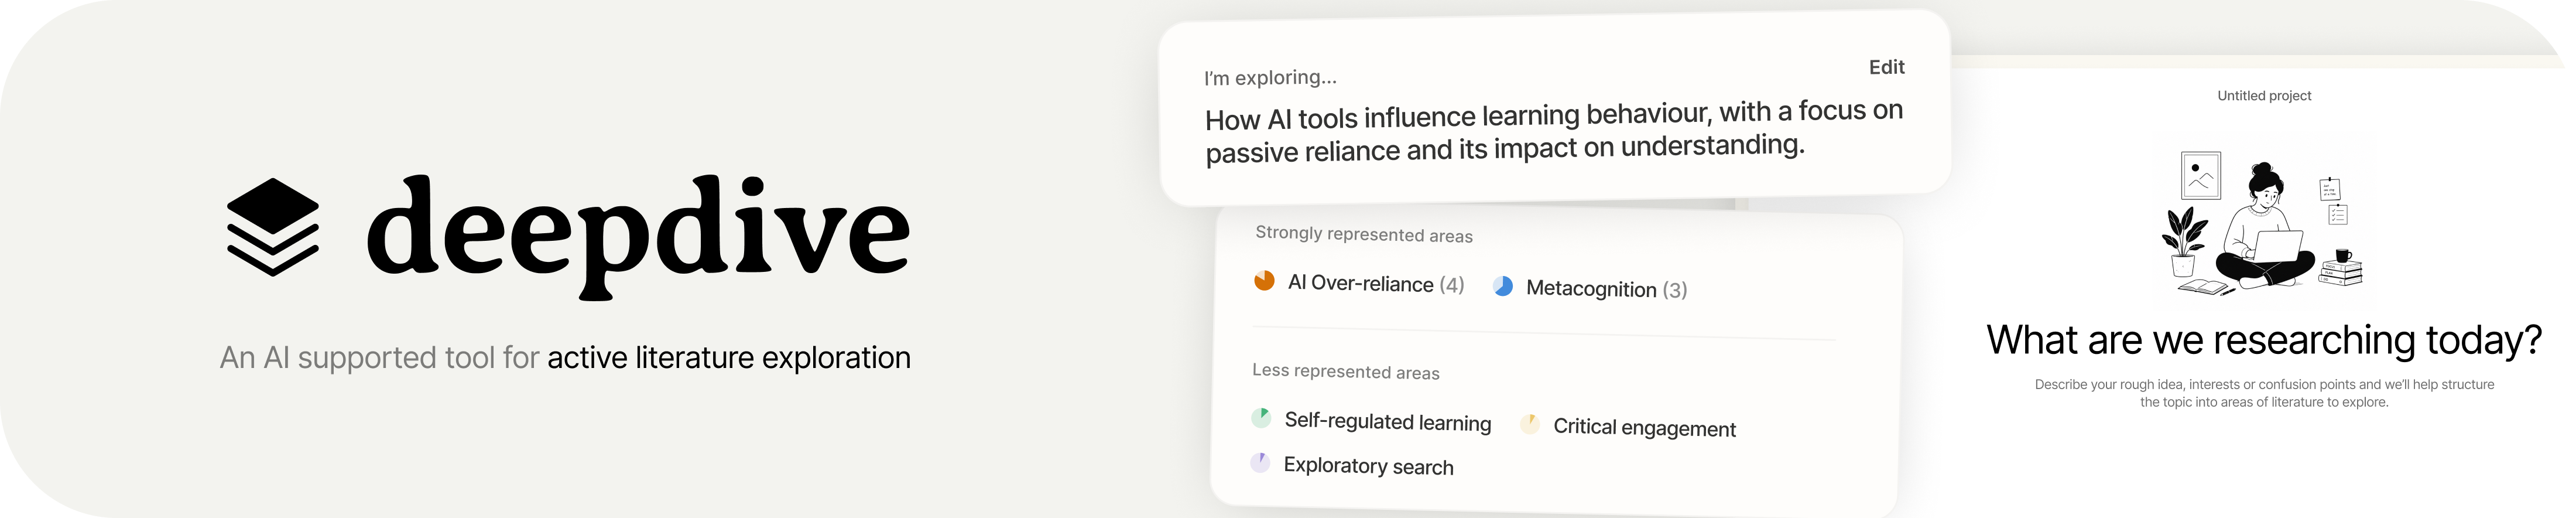
\includegraphics[width=\textwidth]{assets/fig1-teaser}
\caption{DeepDive presents literature exploration as a structured environment rather than a prompt-to-list interaction. The interface foregrounds topic shaping, research-area structure, contribution-framed comparison, and foundation building before citation export.}
\Description{A wide teaser view of the DeepDive interface.}
\label{fig:teaser}
\end{teaserfigure}

\maketitle

\section{Introduction}
AI-assisted literature search has become a common starting point for students beginning a research project. With a short prompt, a system can return lists of papers, summaries, and recommendations almost instantly. This can make literature review feel efficient, but efficiency is not the same as understanding. A student may leave with five apparently relevant papers and still be unable to explain what conversation those papers belong to, what tensions exist between them, or why one paper should be preferred over another. In other words, retrieval can arrive before orientation.

This concern became the starting point for DeepDive. The problem was not framed as whether AI can find literature, because in practice it already can. The more important question was whether the interaction model around retrieval helps the user make sense of what has been found. If an interface collapses the task into a single prompt-to-list step, then the user may be nudged toward selection without synthesis. The result is often a reading list that looks productive on the surface but is weakly understood by the person who assembled it.

This concern aligns with prior work suggesting that AI-generated outputs can feel easier and faster while still producing shallower understanding than more active search practices~\cite{melumad2025llmlearning}. It also aligns with the view that searching is itself a learning process rather than only a retrieval task~\cite{vakkari2016searching}. For literature recommendation systems specifically, explanations and user control matter because users need to understand why items are being recommended, not simply accept that they are relevant~\cite{guesmi2023interactive}. Taken together, these perspectives suggest that the design of the interface around retrieval may matter as much as retrieval quality itself.

This paper presents \textit{DeepDive}, an AI-supported interface for early-stage literature exploration. Rather than collapsing literature review into a prompt-to-list interaction, DeepDive structures the experience into stages: users begin with a rough topic, reflect on what concerns them, confirm research areas proposed by the system, compare papers within those areas, and assemble a literature foundation before citation export becomes available. The design premise is not to automate literature review or produce complete understanding automatically. Instead, the system aims to support conceptual orientation and more intentional paper selection during the earliest stage of review.

The work makes two contributions. First, it presents a design contribution in the form of a structured interaction model for literature exploration. Second, it reports an exploratory evaluation comparing DeepDive with a constrained flat-list baseline. The evaluation focuses on subjective but practically relevant outcomes: perceived understanding, active engagement, confidence, and the ability to articulate why selected papers belong in an initial reading list. The findings are presented as directional patterns from a small course-project study rather than as population-level effects.

\section{Related Work}
\subsection{AI assistance, speed, and shallow understanding}
Recent discussion around AI-supported learning has emphasized a tension between speed and depth. In the framing used throughout this project, the problem is not that AI tools are incapable of helping users find material, but that they can make the process feel complete too early. Melumad and Yun argue that LLM-generated outputs can make learning feel easier while producing shallower understanding than web-search-based learning activities~\cite{melumad2025llmlearning}. This is a useful problem anchor for DeepDive: a user may leave an interaction with a list of papers and a sense of progress while still lacking a usable understanding of the topic structure behind those papers.

For literature review, that distinction matters because the task is not only to obtain sources. Students also need to judge what each source contributes, how sources cluster into areas, and which tensions or gaps those sources reveal. A system that optimizes only for speed may therefore support an early feeling of completion while leaving the harder work of synthesis under-supported.

\subsection{Searching as part of learning}
Vakkari's account of searching as learning reframes information seeking as a process through which understanding develops~\cite{vakkari2016searching}. From that perspective, the interface is not just a container for results. It becomes part of the learning environment itself. Search interactions shape what the user notices, what they compare, and how they represent the space they are entering.

This framing is central to DeepDive. The system deliberately stretches out the moment between initial topic entry and final citation export into a sequence of reflective decisions. The point is not to add steps for their own sake. Rather, the interface attempts to preserve the parts of literature exploration where understanding is most likely to form: clarifying the topic, naming concerns, inspecting conceptual structure, comparing candidate papers, and assembling an intentional reading list.

\subsection{Explanations and control in literature recommendation}
Work on explainable literature recommendation highlights the need for user control and explanations around suggested sources~\cite{guesmi2023interactive}. In such systems, relevance alone is insufficient. A recommendation needs to be legible enough for the user to understand why it appeared and whether it belongs in the current task.

In DeepDive, this principle appears in two ways. First, the system proposes conceptual areas but requires explicit user confirmation. Second, papers are framed by contribution rather than title alone so that the interface foregrounds why a paper might matter. These choices are intended to make the recommendation logic more legible and the user's selection process more intentional. The project therefore extends the logic of explainability from paper-level recommendation toward the level of conceptual structure itself.

\subsection{Implications for this project}
Across these three strands, the same design implication emerges: an interface for AI-supported literature review should not only optimize retrieval accuracy or output speed. It should also make the user an active participant in topic shaping, comparison, and justification. DeepDive adopts that implication directly. Its goal is not to replace judgment but to structure the conditions under which judgment is formed.

\section{DeepDive Design}
\subsection{Design goals}
DeepDive was designed around three high-level goals, matching the framing used in the final presentation. First, it should help users clarify a topic that may still be vague or underspecified. Second, it should make the conceptual shape of the literature visible rather than present a flat list of papers. Third, it should support intentional paper selection by helping users explain why each selected paper belongs in their reading list.

A central design principle is \textit{understanding before extraction}. In the baseline interaction model that DeepDive critiques, retrieval and extraction are effectively immediate: a user asks for papers and can act on the returned list right away. DeepDive instead delays citation export until after users have shaped the topic, explored the research areas, and constructed a literature foundation. The goal is to make understanding a structural part of the interaction rather than a hoped-for byproduct.

\subsection{Workflow overview}
DeepDive structures literature exploration into five main stages: Entry Point, Topic Mapping, Research Area Discovery, Literature Exploration, and Literature Foundation. The presentation materials describe this progression as a movement from a rough topic toward a shaped foundation: users first express an imperfect direction, then map concerns, confirm areas, compare contributions, and finally assemble a structured reading list.

\begin{figure}[t]
  \centering
  \fbox{\parbox{0.94\linewidth}{\centering
  \textbf{Rough topic} $\rightarrow$ \textbf{Map concerns} $\rightarrow$ \textbf{Confirm areas} $\rightarrow$ \textbf{Compare contributions} $\rightarrow$ \textbf{Build foundation}}}
  \caption{Workflow overview of DeepDive. The system restructures early-stage literature review into a sequence of reflective steps rather than an immediate retrieval interaction.}
  \Description{A boxed text workflow overview of the DeepDive process.}
  \label{fig:workflow}
\end{figure}

The importance of this sequence is not that it is longer than a conventional chat interaction, but that each step surfaces a different kind of user judgment. Topic entry allows ambiguity. Topic Mapping turns concerns into explicit signals. Research Area Discovery proposes conceptual structure that can be accepted or contested. Literature Exploration lets users compare papers in the context of those areas. The Literature Foundation makes the emerging reading list visible as a structured object rather than a saved pile.

\subsection{Entry point and Topic Mapping}
The entry point is deliberately simple. Users are not required to begin with a polished research question. Instead, they can start with the kind of partial topic students often have in practice. This low-pressure start was meant to reduce the need to ``perform expertise'' before the system had done any useful work.

The Topic Mapping stage then asks exploratory questions about what concerns the user, what dimensions feel important, and what perspectives they care about. As described in the presentation speaker notes, this design choice intentionally asks users to articulate interests before seeing a set of papers. The interaction is meant to make assumptions visible and to let the user's initial concerns shape what the system proposes next.

\begin{figure}[t]
  \centering
  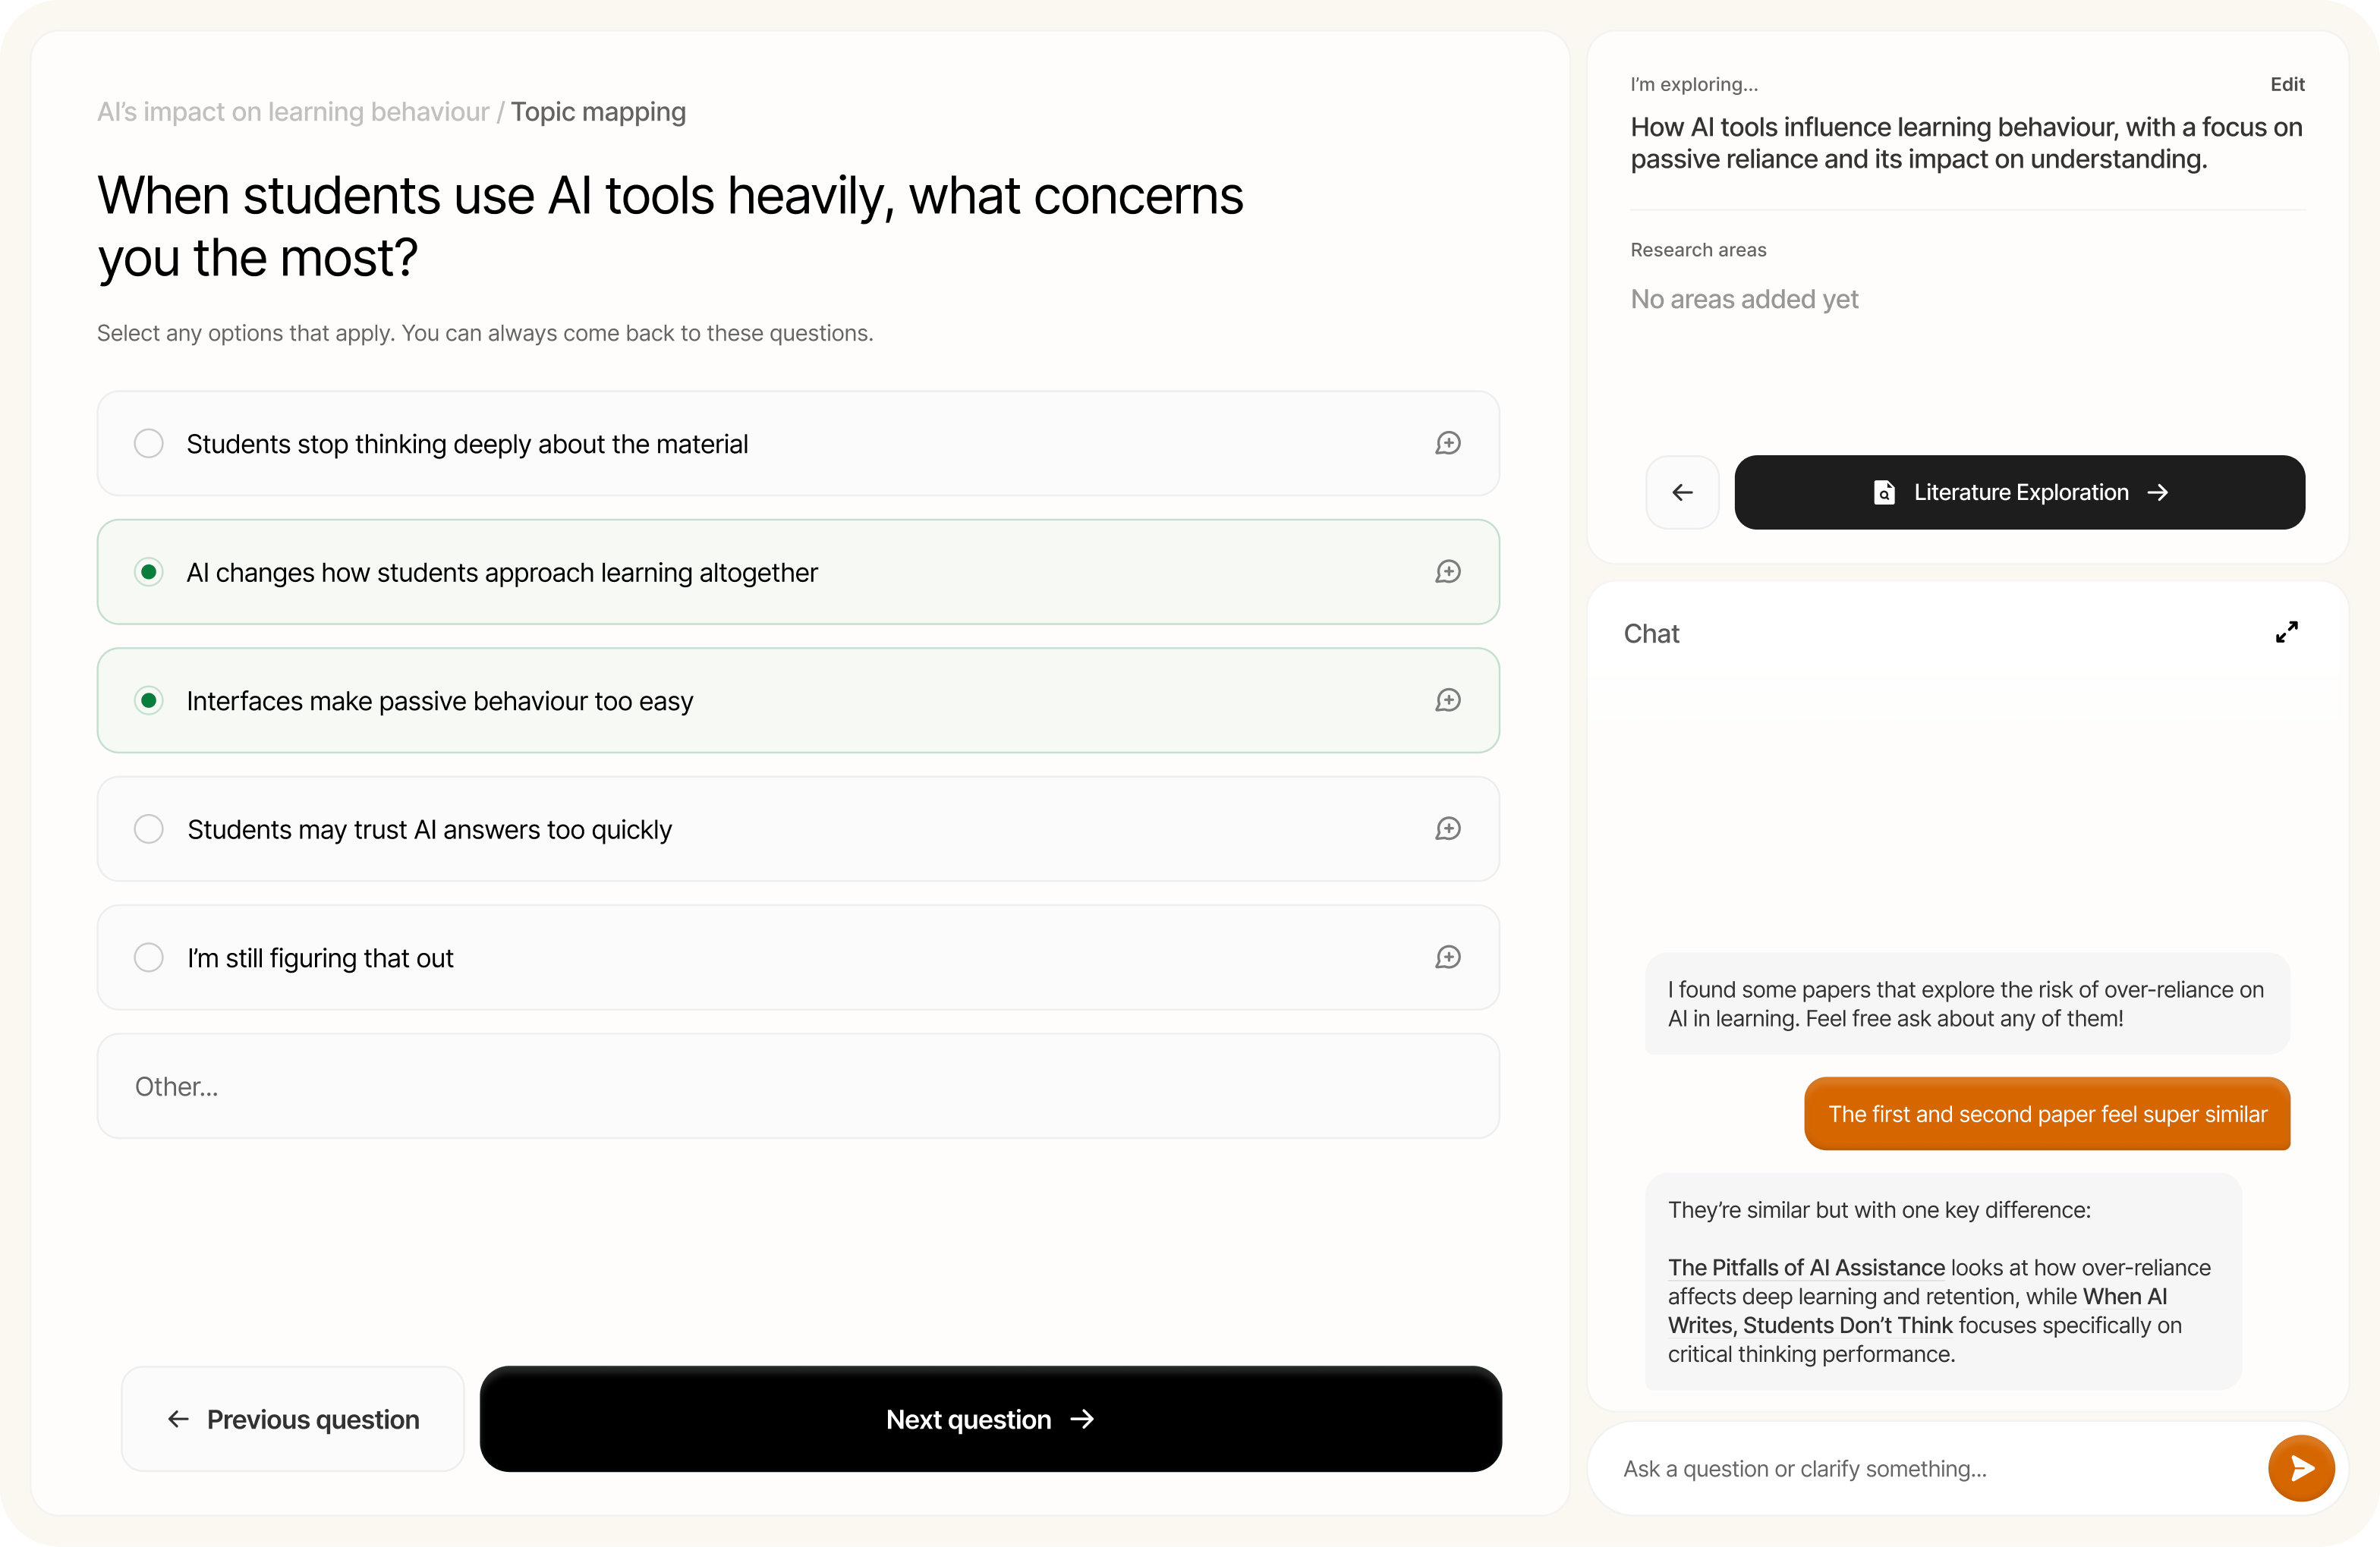
\includegraphics[width=0.92\linewidth]{assets/fig2-topic-mapping}
  \caption{Topic Mapping prompts users to clarify concerns before papers are shown. The step is intended to make assumptions visible rather than let the first retrieved list silently define the field.}
  \Description{The Topic Mapping screen of DeepDive.}
  \label{fig:topicmapping}
\end{figure}

This step introduces one of the design tensions later reflected in the evaluation. For some users, concern-first questioning was perceived as a helpful reflective prompt. For others, especially when the topic already felt clear, it created friction. That tension is important because it shows that structure can support understanding while still imposing a cost on users who feel ready to move directly to sources.

\subsection{Research Area Discovery}
After Topic Mapping, DeepDive proposes conceptual research areas through a modal interaction. The system effectively says: here is one possible way to frame part of your topic. The user then decides whether to add that area to their working map. This was an important part of the project's design philosophy: the system can suggest structure, but it should not silently author the user's conceptual map.

\begin{figure}[t]
  \centering
  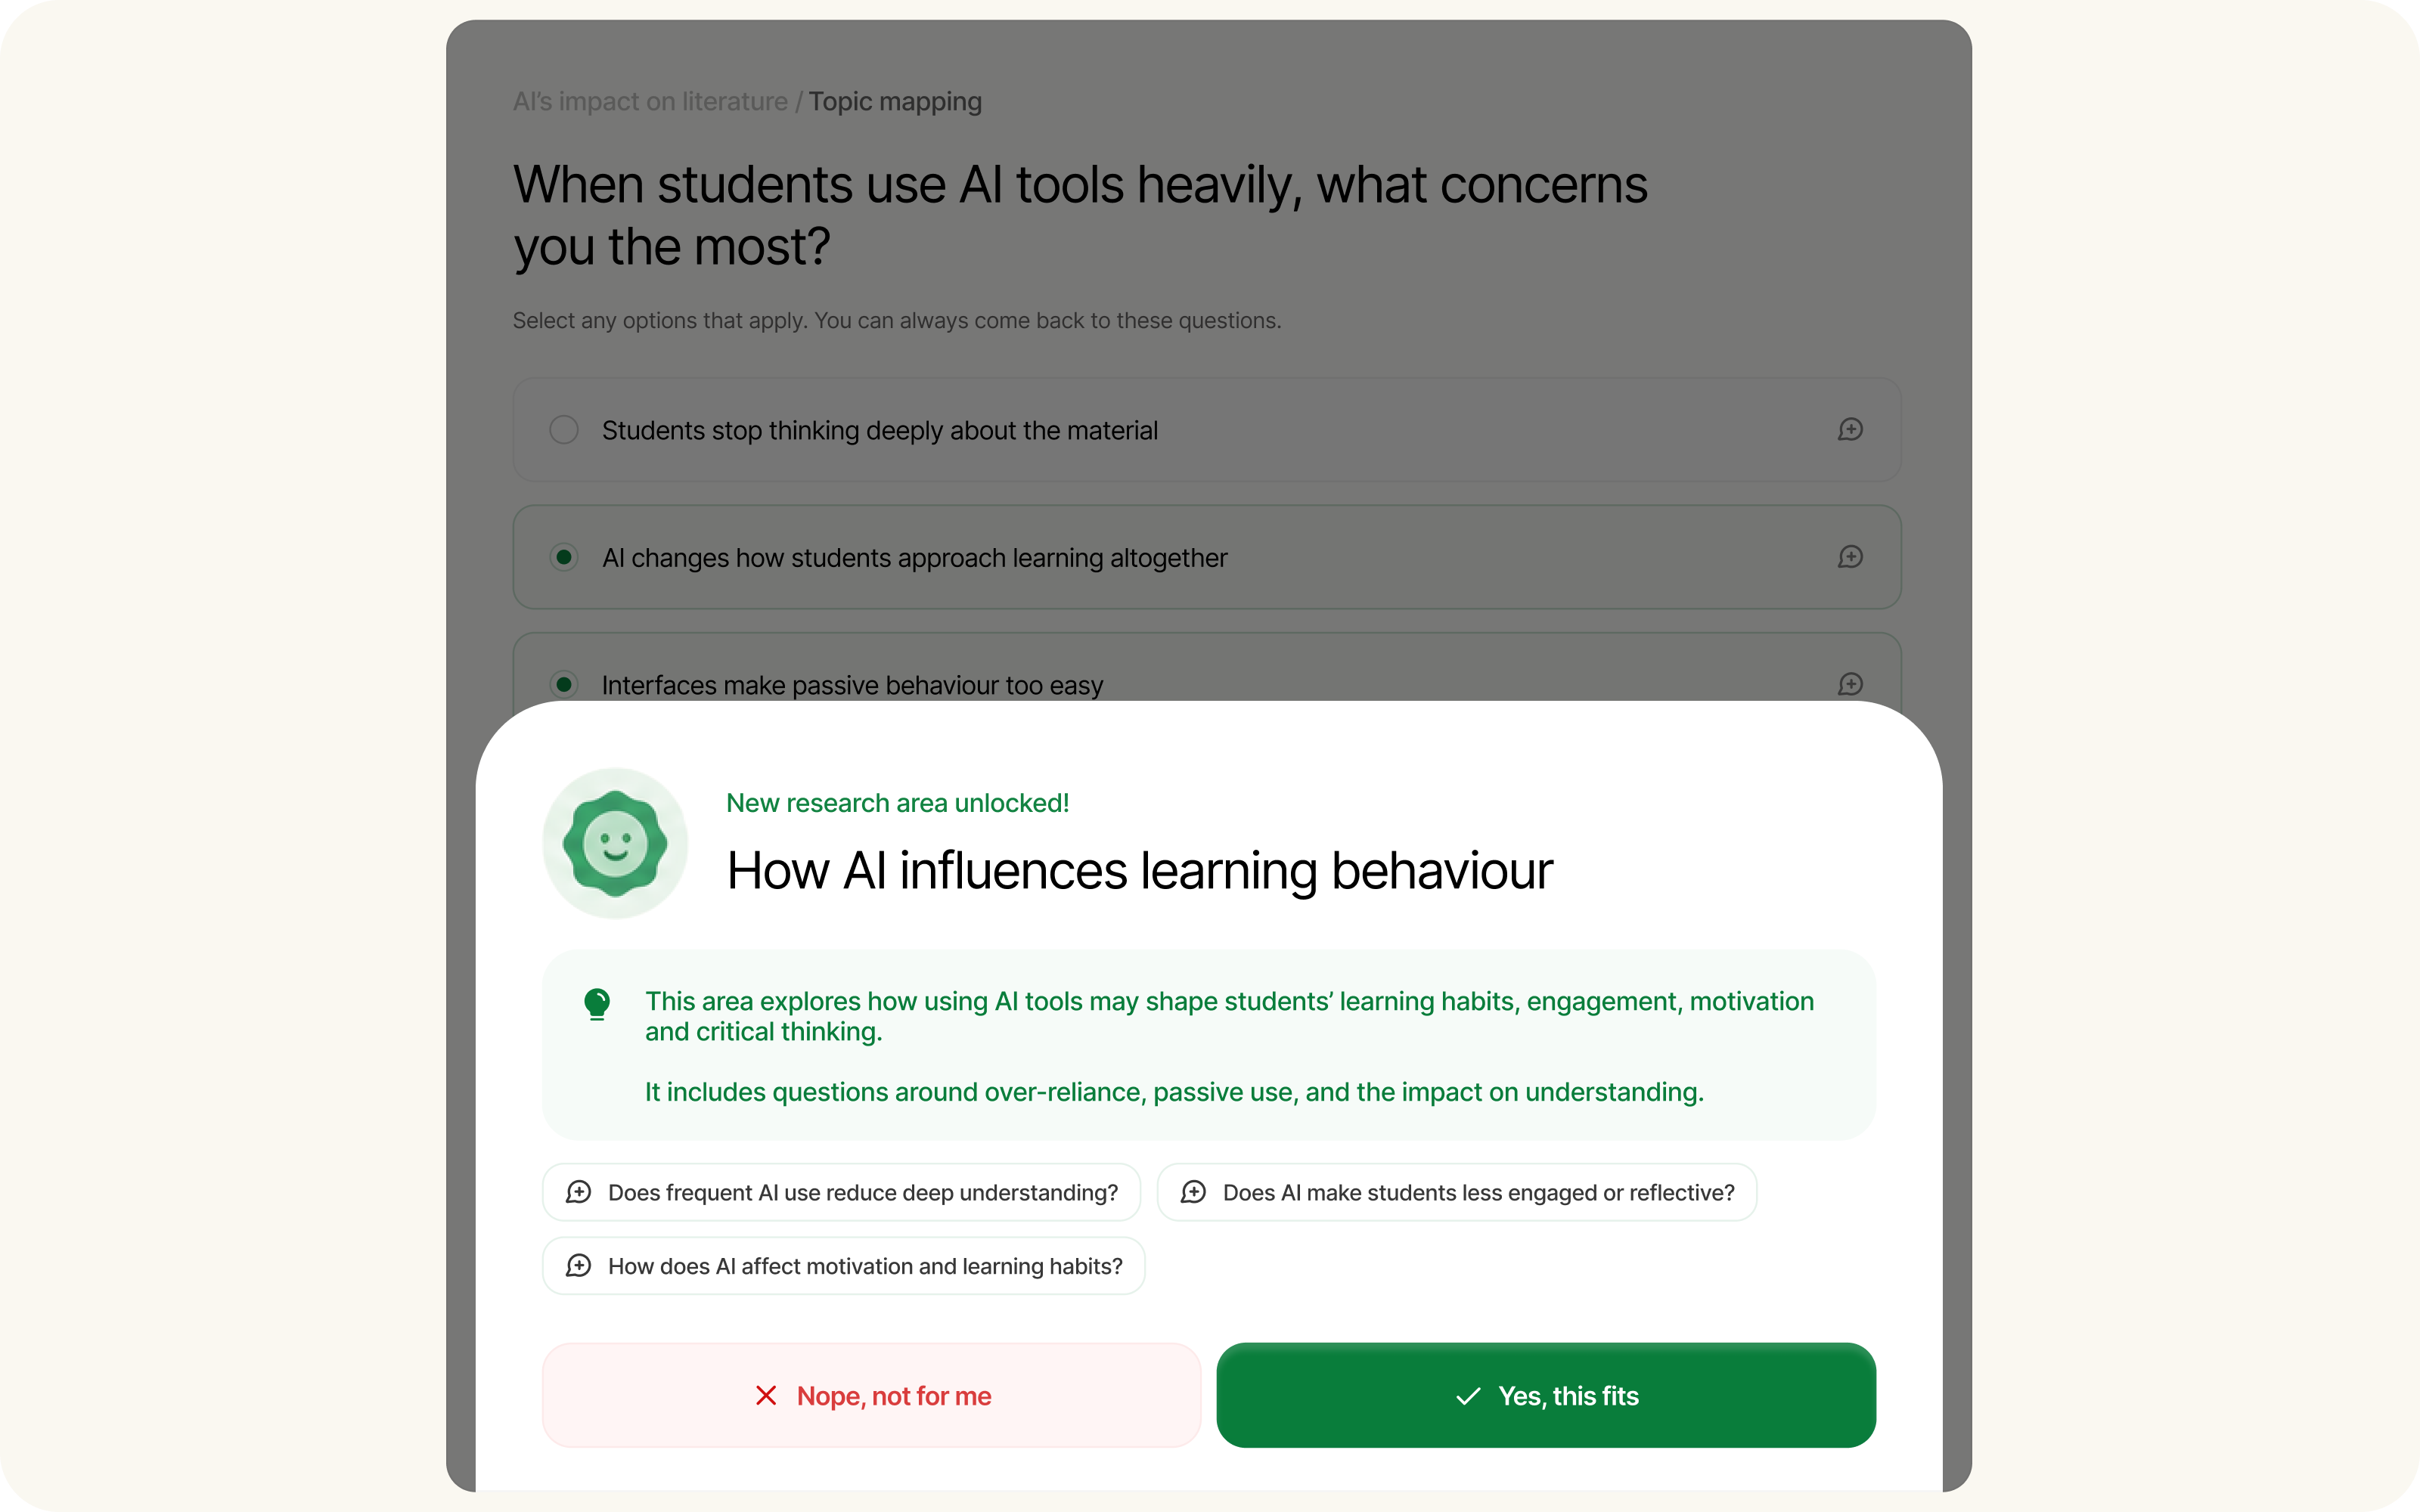
\includegraphics[width=0.92\linewidth]{assets/fig3-area-confirmation}
  \caption{The Research Area Discovery step makes system-authored structure visible and contestable through explicit user confirmation.}
  \Description{The Research Area Discovery modal in DeepDive.}
  \label{fig:areas}
\end{figure}

Two design choices are especially important here. First, the area is presented as a legible conceptual object rather than a hidden internal label. Second, the user-assent gesture matters: the system proposes, but the user confirms. This distinction became meaningful in the evaluation, where participants explicitly noted that the interface preserved a sense of agency by making the structure visible before adoption.

\subsection{Literature Exploration}
Once areas are confirmed, papers appear inside those areas. A key design decision here is that cards foreground contribution rather than title. In the project's presentation, this was framed very directly: a title tells the user what a paper is called, while a contribution helps the user judge why it might matter at this early stage of a review. The design therefore tries to support comparison not at the level of surface relevance, but at the level of what each paper offers to the emerging understanding of the topic.

\begin{figure}[t]
  \centering
  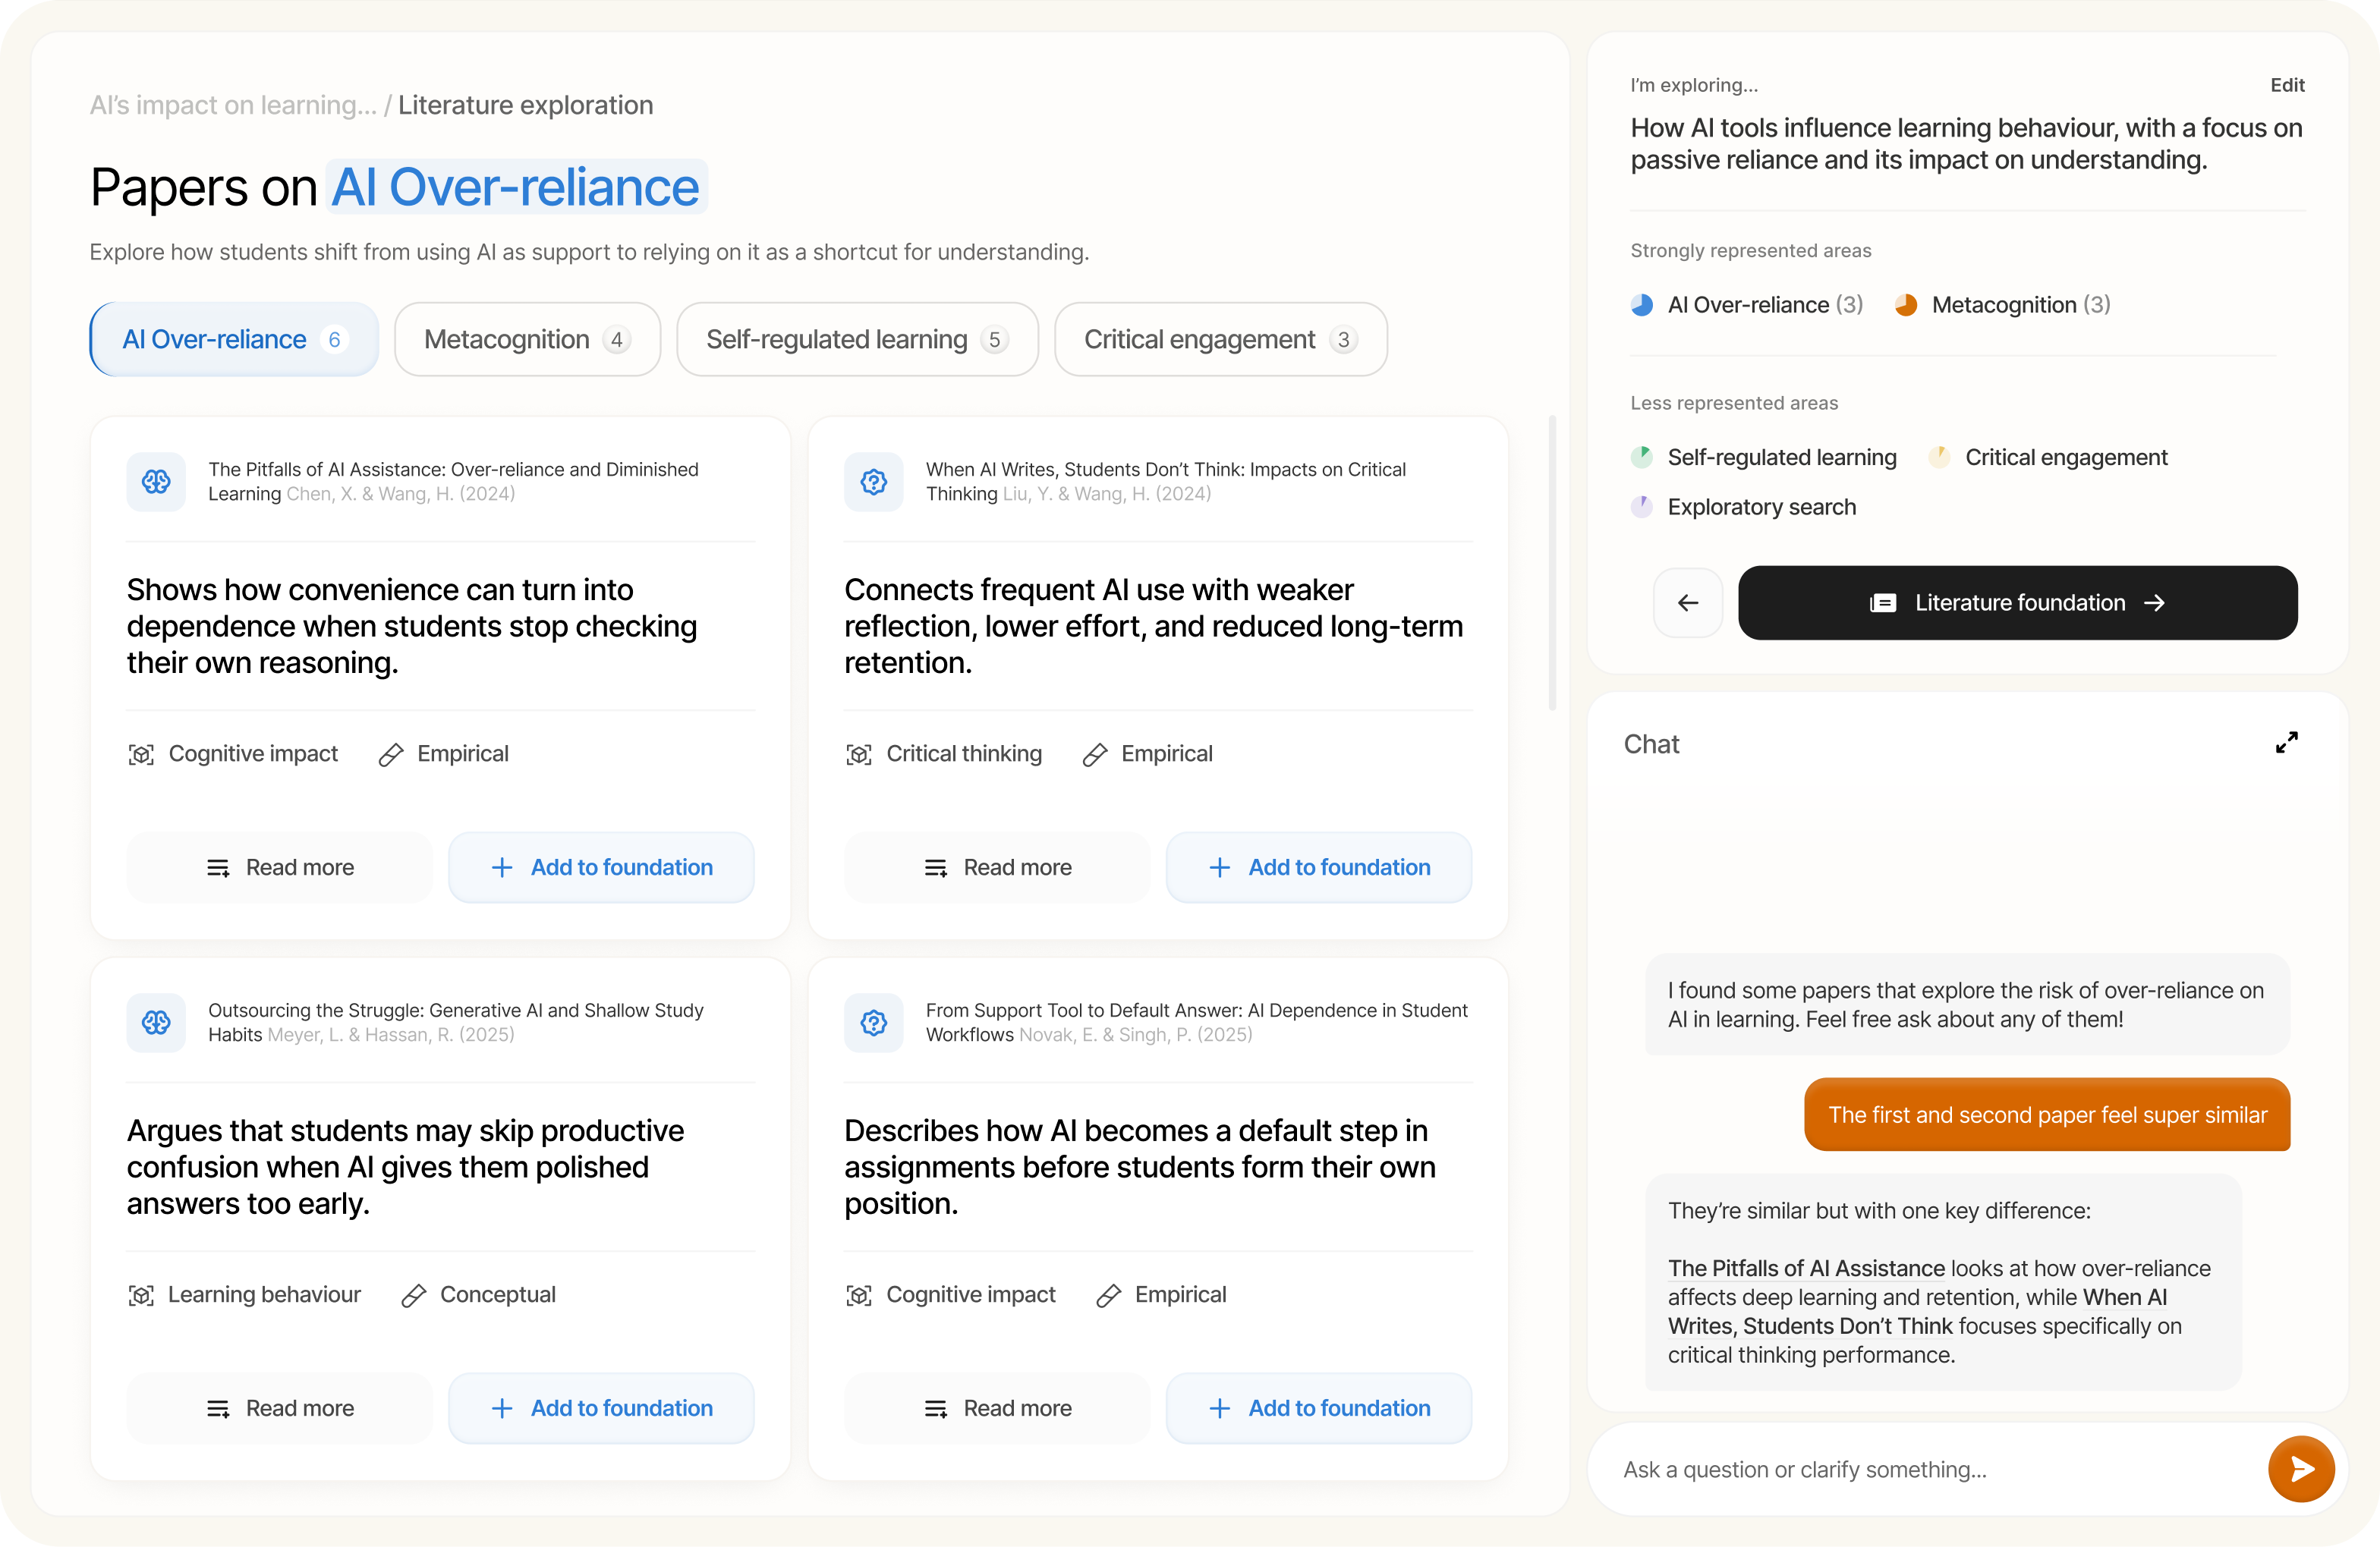
\includegraphics[width=0.92\linewidth]{assets/fig4-literature-exploration}
  \caption{DeepDive's Literature Exploration view organizes papers by confirmed areas and frames them by contribution rather than title alone.}
  \Description{The Literature Exploration view of DeepDive.}
  \label{fig:exploration}
\end{figure}

The exploration screen also maintains a visible sidebar representation of the growing foundation. This gives the user awareness of which areas are being represented and which remain lighter. Importantly, the balance indicator is not intended to prescribe a correct distribution. Its purpose is to make the shape of the reading list visible enough for the user to inspect and possibly respond to.

\subsection{Literature Foundation}
The Literature Foundation screen groups the selected papers by area and only then exposes citation export. This screen operationalizes the principle of understanding before extraction by turning the reading list into a structured foundation rather than a flat pile of saved citations.

\begin{figure}[t]
  \centering
  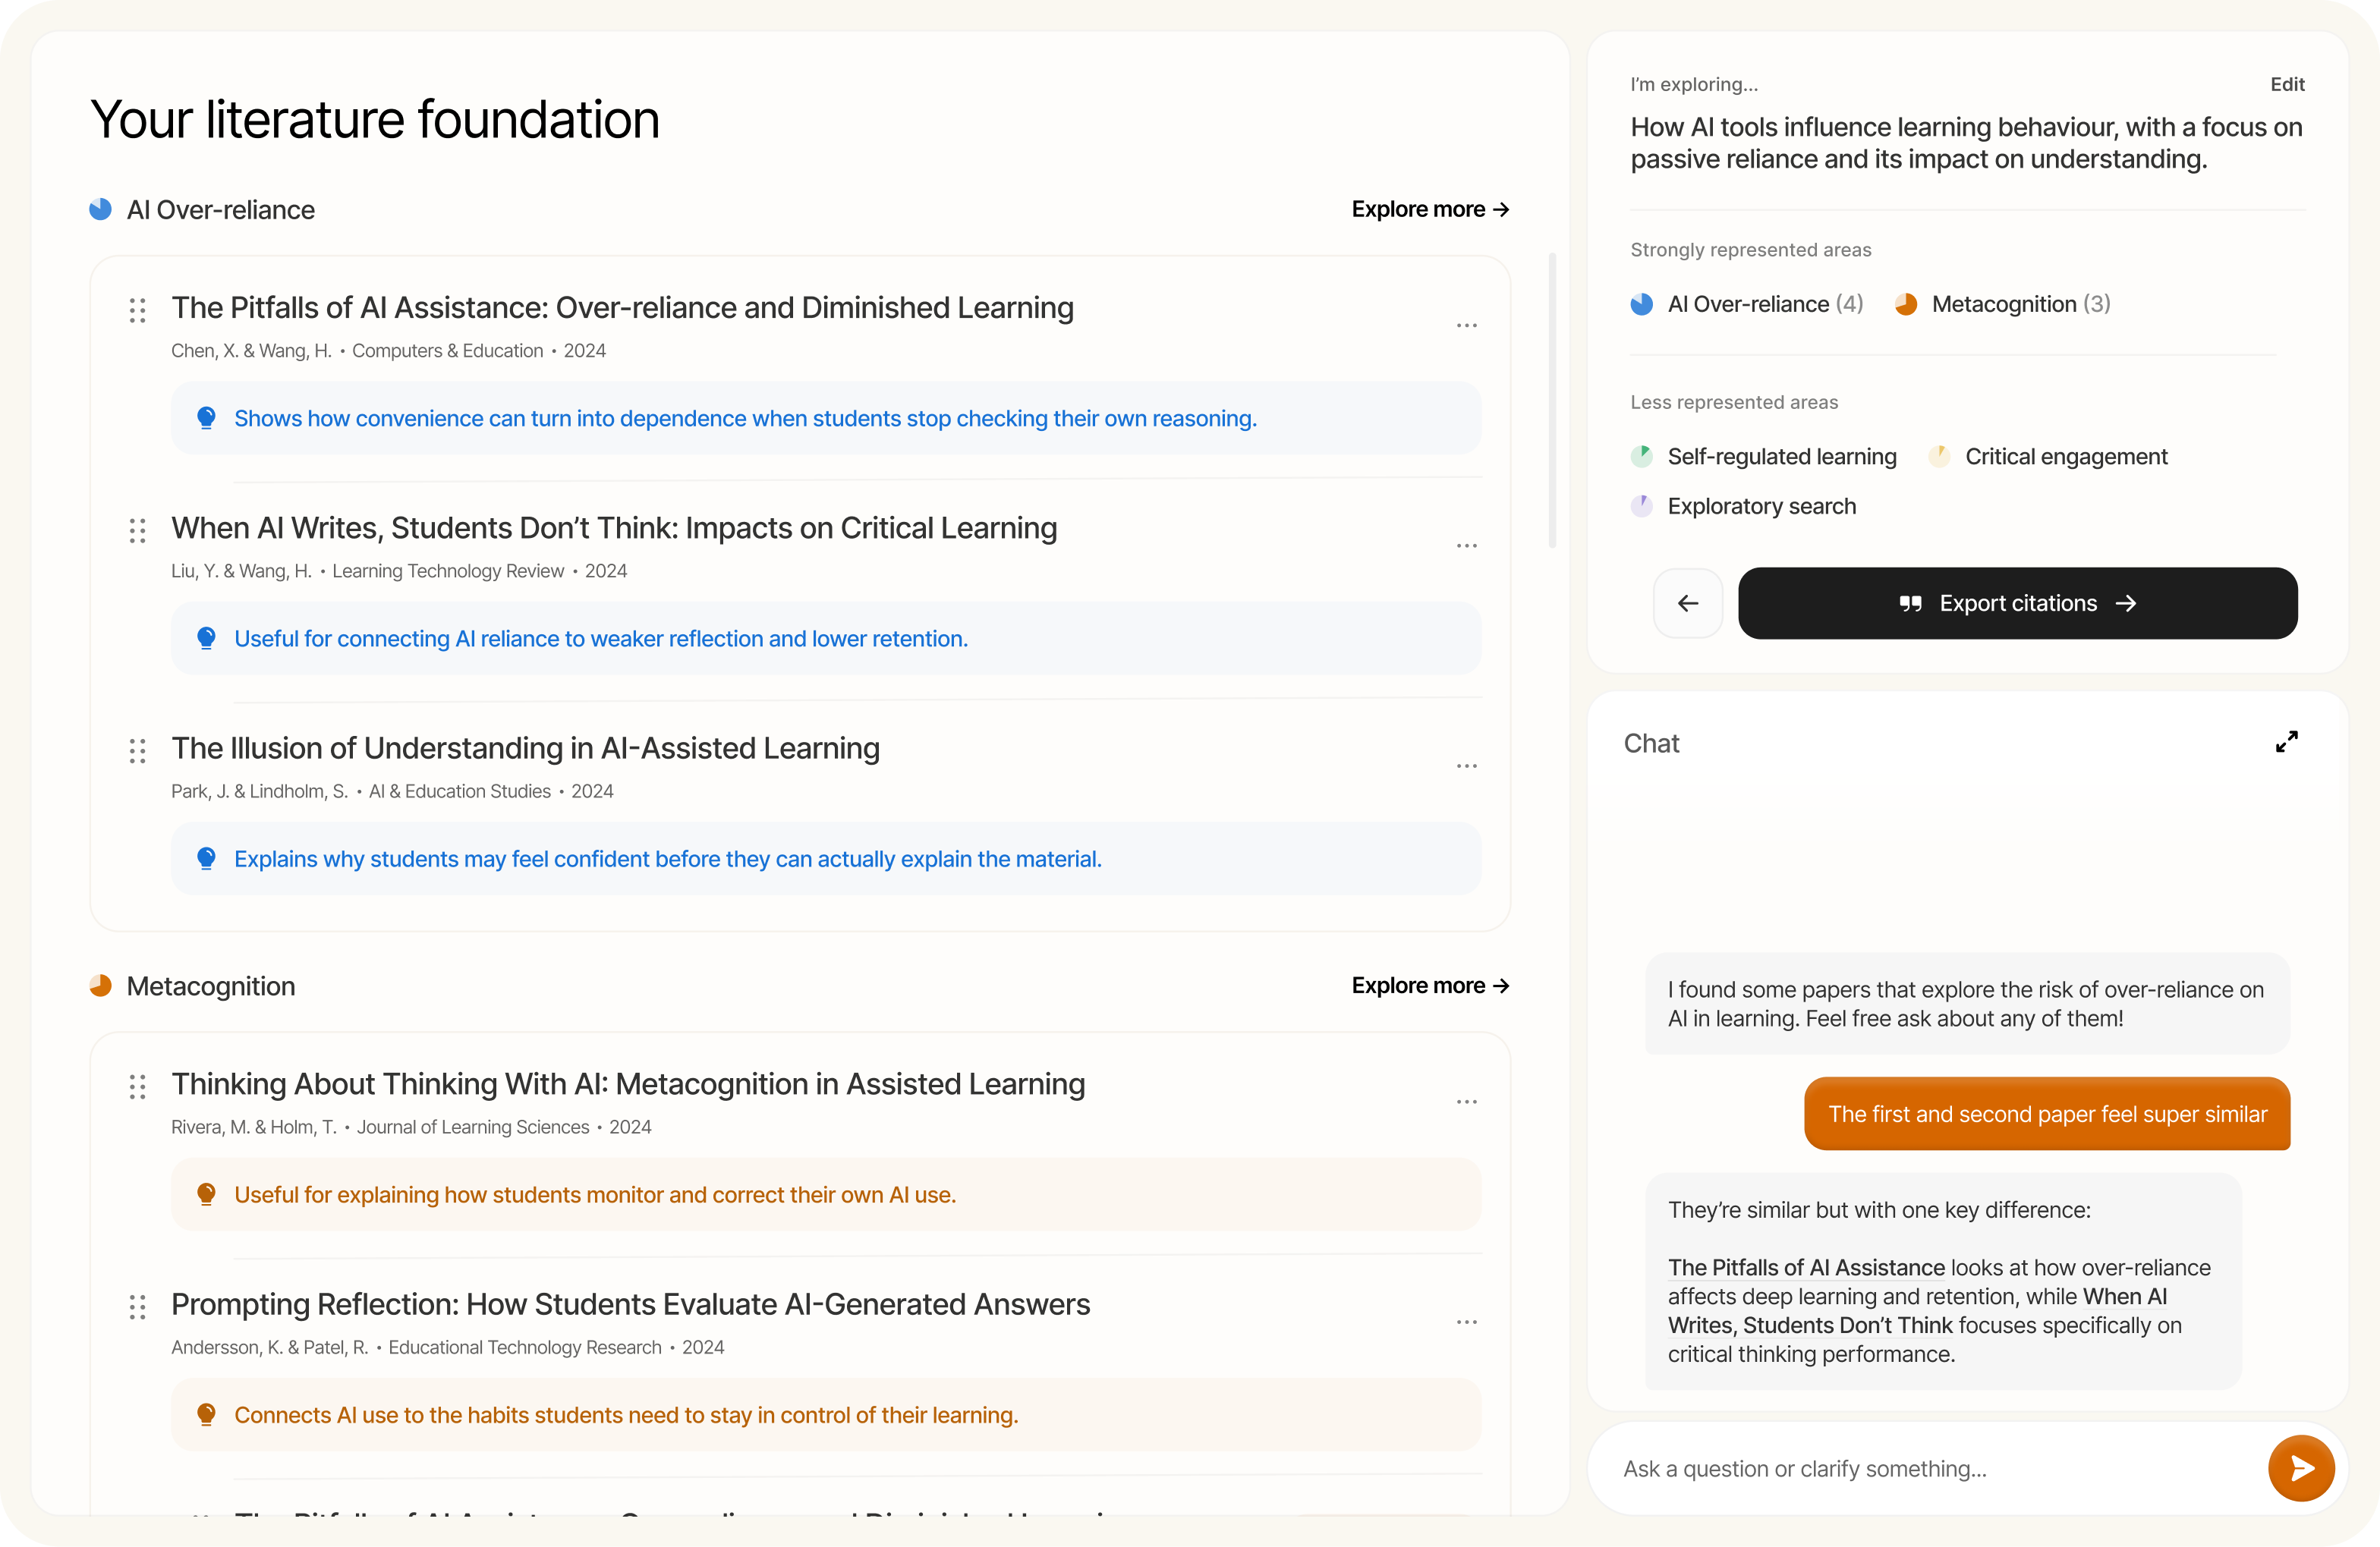
\includegraphics[width=0.92\linewidth]{assets/fig5-foundation}
  \caption{The Literature Foundation screen assembles a structured reading list and places citation export after exploration rather than before it.}
  \Description{The Literature Foundation view of DeepDive.}
  \label{fig:foundation}
\end{figure}

This final state reframes the output of the interaction. The user is not merely leaving with links. They are leaving with a set of papers whose grouping, relative coverage, and contribution to the topic have already been made part of the selection process.

\section{Method}
\subsection{Study design}
The evaluation asked whether a structured exploration workflow would affect participants' confidence in their literature selections and their ability to articulate why those selections mattered, compared to an unstructured AI-retrieval baseline. To study this, DeepDive was compared with a constrained flat-list baseline in a within-subjects, counterbalanced design. Each participant completed both conditions, with topic order crossed against condition order.

The baseline was intentionally constrained in order to compare two interaction models on more balanced terms: immediate retrieval versus structured exploration. In the baseline condition, participants received a flat list of papers with titles and short excerpts, without Topic Mapping, Research Area Discovery, or contribution-framed organization. In the DeepDive condition, participants moved through the staged workflow described above. Because both interfaces were prototypes, the baseline did not fully reproduce the responsiveness participants might associate with a production chatbot. This is both a limitation of the implementation and a consequence of the study's scope-matching design choice.

\subsection{Participants and task}
Five master's-level students known to the researcher volunteered to participate. All were enrolled in master's-level courses and had prior exposure to academic literature. The study used convenience recruitment rather than random sampling, which fits the scope of the project but also constrains the claims that can be made from the results.

Participants completed the same high-level task in both conditions: select three to five papers for an initial reading list on an assigned topic. The two topics were drawn from the same meta-domain and the same underlying paper pool was used across conditions so that the comparison stayed focused on interaction structure rather than content availability. This choice was important because it prevented differences in surfaced content from overwhelming the design comparison.

\subsection{Procedure}
Each participant completed one topic per condition and was asked to think aloud while working. After each condition, participants rated confidence, articulation, perceived understanding, and active engagement on a five-point Likert scale. They also responded to an open-ended articulation prompt asking them to describe the research area, explain how the selected papers related to it, and justify why those papers had been chosen.

At the end of the session, participants also answered comparative questions about which condition helped them understand the topic better and which they would trust more for a real assignment. These comparative questions were useful because they captured participants' holistic judgments after encountering both interaction models.

\subsection{Data sources and analysis}
Think-aloud observations were captured through session notes and supported by recordings and transcription. Quantitative analysis remained descriptive: per-item means and condition differences were summarized without statistical inference. This matched the scale of the project and avoided overstating what could be concluded from a five-participant sample.

Qualitative material was coded thematically over multiple passes using the dimensions defined in the evaluation protocol: structural understanding, comparison-based reasoning, and intentionality cues. The purpose of the qualitative analysis was not to produce an exhaustive coding schema, but to test whether the kind of articulation encouraged by DeepDive differed noticeably from the kind of articulation produced under the baseline.

\section{Results}
\subsection{Quantitative pattern}
Across this sample, DeepDive produced higher mean ratings on all four measured items than the constrained baseline. The strongest shifts were in active engagement, perceived understanding, and articulation, while confidence increased more modestly. This pattern matches the framing used in the project presentation: the important change was not simply that users felt more confident, but that they were better able to explain why selected papers belonged in their reading list.

\begin{table}[t]
  \caption{Mean ratings by condition (1--5 scale, $n=5$).}
  \label{tab:means}
  \centering
  \begin{tabular}{lccc}
    \toprule
    Item & Baseline & DeepDive & Difference \\
    \midrule
    Confidence & 3.2 & 4.2 & +1.0 \\
    Articulation & 2.4 & 4.4 & +2.0 \\
    Perceived understanding & 2.0 & 4.2 & +2.2 \\
    Active engagement & 2.0 & 4.4 & +2.4 \\
    \bottomrule
  \end{tabular}
\end{table}

The largest shift appears on active engagement (+2.4), followed closely by perceived understanding (+2.2) and articulation (+2.0). Confidence also increased, but by a smaller margin (+1.0). This matters because it suggests that the main value of the interface was not simply producing a stronger feeling of certainty. Rather, it supported richer understanding and stronger justification.

The confidence item also behaved somewhat differently from the others. In the findings notes, one participant explicitly remarked that confidence itself had not changed much because they were generally confident in their selections regardless of interface, whereas the articulation gap was where the real difference showed up. This distinction helps interpret the table: confidence can remain relatively high even when the explanatory basis for that confidence is weak.

Five of five participants reported equal or higher scores on every measured item under DeepDive; no participant rated any item lower under the structured condition. In comparative judgments, all five participants reported that DeepDive helped them understand the topic better, and all five said they would trust it more as a starting point for a real assignment, though every trust judgment came with a caveat.

\subsection{Comparative judgments and behavioural traces}
The behavioural traces from DeepDive provide a useful complement to the Likert ratings. All five participants surfaced and confirmed four research areas. Four of five explored every confirmed area. Four of five selected papers from at least three areas, and three of five selected across all four. The balance indicator was noticed by all five participants, but only one participant clearly changed a selection in response to it. For the others, it functioned more as a representational cue than a direct behavioural prompt.

This matters because it shows that some design elements were doing perceptual work even when they did not immediately produce action. The sidebar did not strongly dictate selection behaviour, but it kept the shape of the foundation visible. That alone changed how users talked about their reading list, which is consistent with the broader articulation findings.

\subsection{Qualitative articulation shift}
The clearest qualitative shift appeared in participants' open-ended explanations. Under the baseline, several responses stopped at relevance: papers matched the topic, seemed appropriate, or looked like reasonable starting points. Under DeepDive, participants more often described sub-areas, tensions between papers, and the specific role individual papers played in the broader topic. In other words, the explanations became more structural and comparative.

The findings notes coded articulation along three dimensions: structural understanding, comparison-based reasoning, and intentionality cues. Under the baseline, three of five participants were rated absent on both structural understanding and comparison-based reasoning. The two stronger baseline articulations came from participants who explicitly attributed that structure to their own prior knowledge rather than to the interface. Under DeepDive, all five participants reached the strongest rating on all three dimensions. The articulation difference is therefore not a subtle one in the transcripts. It is the single clearest qualitative shift in the study.

Two interface elements carried most of the qualitative weight. First, contribution-framed cards helped participants compare papers on the basis of what each paper offered rather than what it was called. Second, the area-discovery step gave participants a vocabulary for discussing the shape of the research space. In the findings notes, one participant described the area modal as the moment ``where it clicked,'' while another emphasized that the structure helped turn papers into positions in a conversation rather than a pile of related items.

\subsection{What seemed to work}
Four design moves seemed to carry most of the weight in the evaluation.

\begin{itemize}[leftmargin=1.5em]
  \item \textbf{Contribution-framed cards.} Four of five participants named this, often unprompted, as the most useful design choice. It supported comparison at the level of contribution rather than title recognition.
  \item \textbf{Research areas as structure.} The area-discovery step repeatedly appeared in participant accounts as the moment where the topic became thinkable in pieces rather than as a flat pile of related papers.
  \item \textbf{User confirmation of areas.} Participants noticed that the system did not silently impose the map. The act of accepting or rejecting proposed areas helped preserve a sense of agency.
  \item \textbf{Foundation as a constructed output.} The final screen framed the reading list as something built through choices rather than something simply returned by the system.
\end{itemize}

These points align closely with the original design rationale. The study does not merely show that users liked the system more. It shows that the specific moves the project was built around were the same ones participants later described as carrying the interaction.

\subsection{Critiques and caveats from participants}
The evaluation also surfaced a coherent set of critiques. Participants noted that Topic Mapping could do more priming work than the design explicitly acknowledged, especially when the offered options constrained how a topic was framed. Others suggested that system-authored areas risk becoming a \textit{soft cage} unless users can add or reshape the conceptual structure themselves. A related critique concerned trust relocation: the design may reduce over-trust in paper lists while increasing trust in the system's ontology of the field. Finally, participants who already felt clear about their topic found the survey step more frictional, and the chat sidebar was sometimes perceived as secondary or vestigial.

These critiques are important to the value of the evaluation rather than incidental to it. They help define the design space around structured exploration: structure can scaffold understanding, but it must remain contestable and flexible enough not to harden into an unquestioned map.

\section{Discussion}
The evaluation suggests that the main value of DeepDive lies in helping users move from selecting papers that look relevant to articulating why specific papers belong together in an early-stage reading list. This aligns with the core framing used throughout the presentation and report notes: the problem is not just retrieval quality, but the interaction model surrounding retrieval.

\subsection{From relevance to explanation}
One useful way to interpret the results is through an articulation--confidence gap. In the baseline condition, participants could often feel that their paper choices were acceptable, but their explanations remained thin. In the DeepDive condition, confidence also increased, but the more meaningful change was that users produced richer and more comparative justifications. This suggests that structured exploration may support a more active relationship to the literature even when it does not simply maximize speed or convenience.

This distinction also clarifies why the open-ended articulation prompt mattered so much in the evaluation. Confidence alone can be misleading. A person may feel that a list looks good because the titles appear relevant or familiar. The articulation prompt forces a different standard: can the user actually describe the space, explain the roles papers play within it, and justify the composition of the reading list? On that measure, the difference between the two interaction models became much more visible.

\subsection{Structure as scaffold, not cage}
At the same time, the evaluation makes clear that structure is not automatically beneficial. Several of the strongest participant critiques concern the risk that structure might narrow thought too early or encourage misplaced trust in the system-authored decomposition of a topic. In the language used in the presentation, the lesson is that structure should function as a scaffold, not a cage.

This has two implications. First, the conceptual map needs contestability. It is not enough for the user to confirm individual areas if the overall decomposition itself may be wrong. Second, the interface should support user-authored structure, especially in cases where the user's actual question sits between suggested areas or outside them entirely. The same design feature that supported orientation in this study could become a source of misdirection if the ontology were poor.

\subsection{Design implications}
The findings point toward several concrete next steps for the design:

\begin{itemize}[leftmargin=1.5em]
  \item add an ``add your own area'' affordance so that the structure can be co-authored rather than merely confirmed;
  \item provide a pathway for saying that the decomposition itself feels off, not just that one proposed area should be rejected;
  \item make Topic Mapping skippable or compressible for users whose topic already feels clear;
  \item either strengthen the role of the chat sidebar or remove it if the structured workflow is doing nearly all of the work;
  \item surface more provenance around suggested areas so users can calibrate trust in the system's framing.
\end{itemize}

These are not generic feature requests. They emerge directly from the evaluation and help explain where the design succeeded and where it remains fragile.

\subsection{What this study can and cannot say}
The results should be read as directional. With five participants, single-session use, and self-report-heavy measures, the study cannot support strong general claims. It also cannot show that DeepDive produces objectively better literature reviews or objectively better paper choices. Multiple design features were bundled together in the DeepDive condition, so the study cannot isolate whether the observed differences came primarily from area structure, contribution framing, or another component.

What the study can say is narrower but still useful: in this sample, every participant judged DeepDive better for understanding the topic, every participant gave it equal or higher ratings on every measured item, and the open-ended explanations under DeepDive were visibly more structured and comparative. The study therefore offers a credible course-project-level argument that interaction structure influences how users understand and justify literature choices.

\section{Limitations and Conclusion}
This study has several important limitations. It involved a small convenience sample of five participants, relied heavily on subjective measures and self-report, and took place in a single session. The baseline condition was intentionally constrained and therefore does not represent the full capability of a production conversational AI system. Demand characteristics are also relevant because participants knew they were comparing two interfaces designed by the researcher. In addition, multiple design features were bundled together in the DeepDive condition, so the study cannot isolate whether the observed differences were driven more by area structure, contribution framing, or another interaction component.

A further limitation is that the study did not test failure cases in which the system's proposed ontology is poor or misleading. Several participants correctly identified this as an important unknown. The current findings therefore speak most directly to cases where the proposed area structure is plausible enough to support orientation rather than misdirect it.

Within those limits, the findings still support a useful conclusion for the scope of this project. DeepDive suggests that an AI-supported interface for literature exploration can be designed around active understanding rather than immediate extraction. In this sample, participants using DeepDive reported stronger perceived understanding, higher engagement, and better ability to articulate their paper choices than when using a constrained flat-list baseline. Just as importantly, the evaluation surfaced concrete design tensions around priming, contestability, and trust that should shape future iterations of structured literature exploration systems.

\begin{acks}
This report documents a course project in AI for Learning at KTH Royal Institute of Technology. Bibliographic verification should be completed before final submission for any sources added beyond the current audited set.
\end{acks}

\bibliographystyle{ACM-Reference-Format}
\bibliography{references}

\end{document}
